\chapter{Assembling programming environment}
\label{ch:prog_env}

Source code editor, compiler and debugger are the fundamental development tools.  Hardware project also require a chip programmer, which loads code and configuration from PC to a microcontroller. These tools, along with other useful utilities are referred as a programming environment. They allow to create and build code for a device.

However, when a code is first written, more often than not, it does not work as expected. Unit testing helps, but often errors arise from making false assumptions and these may be reflected in tests as well. In such case, only observing the actual behaviour during execution will lead to fixing the issue. But how to observe the behaviour of a wireless sensor node after it has been flashed with a new executable image? One way is to observe LEDs or an LCD of the device, but only a small amount of information can be retrieved through through such a channel. The debugger is an another option, but by far the most convenient way is to send messages from the MCU to the PC's console.

Existing tools were able to provide most of the needed functionality, however, some of them required project specific configuration, because none of the tools were previously tested with Chronos.

\section{MSPDebug}
\label{ch:mspdebug}

MSPDebug\footnote{MSPDebug: \url{http://mspdebug.sourceforge.net/} created by Daniel Beer} is a debugger and a chip programmer for MSP430 microprocessor architecture.
It is a manufacturer-independent, open source implementation of few debugging protocols.
It requires one of the supported hardware programmers: RF2500, FET430UIF, LaunchPad, Olimex MSP430-JTAG-TINY or MSP430-JTAG-ISO.

% FET, SPI wire programming, JTAG
The eZ430 programmer is called Flash Emulation Tool (FET).
It is connected to PC through USB and to eZ430 Chronos watch through Spy-Bi-Wire (SPI). 
SPI is a two-wire serialised variant of Join Test Action Group (JTAG) protocol.

Despite MSPDebug claimed to support eZ430-FET chip programmer, the version 0.16-1 available in Ubuntu 11.04 does not work with our hardware Luckily, the most recent version of code from project's repository does not have this flaw.

\subsection{Bugs}
\label{ch:mspd_bugs}
In addition to that, the programs on eZ430 could not be resumed correctly by the debugger.
We fixed this bug by correcting one of the constant value.

\subsection{Limitations}
\label{ch:mspd_limitations}

% Transfer speed
Programming the Chronos is rather slow. While it is possible to increase the speed by manually setting the transfer block size, this also increases the risk of programming failure.

Experimentally, we found the 256 bytes blocks as a good trade-off between stability and performance.

This parameter can be modified in \texttt{~/.mspdebug} file by adding the following configuration line:

\texttt{opt fet\_block\_size 256}


\section{Printf library}
\label{sec:printf_library}

TinyOS has a convenient printf library that allows a sensor node to send text messages to the PC, to which the node is connected. The messages are then received by a client application running on the PI, which subsequently displays them on a console. To use the library the following steps are necessary:

\begin{itemize}
  \item Including the printf library files to the sensor node  build, by adding the following line to a Makefile:

    \texttt{CFLAGS += -I\$(TOSDIR)/lib/printf}

  \item Optionally, increasing the printf buffer size (250 bytes by default), by adding the following line to the Makefile:

    \texttt{CFLAGS += -DPRINTF\_BUFFER\_SIZE=<NEW\_SIZE>}

  \item Instantiating printf components in the debugged application configuration. This step depends on which implementation of printf is used. See the following sections for details.

  \item Adding the following include directive in the file from which printf is used:

    \texttt{\#include ``printf.h''}

  \item Using \texttt{printf} statement in the file to display messages and occasionally \texttt{printfflush} to ensure that they are not stuck in a buffer.

    \texttt{printf(``Value is \%d\textbackslash n'', value);} \\
    \texttt{printfflush();}

  \item To receive the messages, the aforementioned printf client, has to be run on the PC. How this is done also depends on the implementation of printf.
\end{itemize}

Before we delve in to the specific implementations of printf, note the following limitation of the mechanism. Only after the buffer is halfway filled or when \texttt{printfflush} is called, does the data get actually sent to the PC. This, however, doesn't happen immediately. If quickly afterwards more text than the capacity of the buffer is printed, some of the text will be lost. Moreover, \texttt{printfflush} is non-blocking, and after returning, the buffer can still be full, and text may get lost. Such a limitation is a consequence of the TinyOS concurrency model, which we discuss in detail in Section \ref{sec:interrupts_and_async}.

To overcome this, a single task should not print more text then the buffer space.

\subsection{MSPDebug printf}
\label{ch:mspd_printf}

Our first approach utilize MSPDebug.
It is a debugger capable of stopping/starting a program and dumping/uploading device RAM to connected PC.

The idea was to create an buffer in eZ430 RAM, where printf would store its output.
The debugger from PC would periodically stop the code execution, fetch the buffer content and reset its size.

The implementation is fully functional, but has two important limitation.
The debugger operations are slow, which limits the feasible printf output rate.
Moreover, stopping the code execution interferes with timers.
This leads to errors in device drivers, if the stop occur during the driver function execution.

This was our first printf library, which allowed to debug basic programs, but was not very useful in debugging more complicated code.
Later, we discontinued this approach, because next methods are superior in all of our scenarios.

\subsection{Radio printf}
\label{ch:radio_printf}

% just use radio and gnode

At some point of the project, we had functioning radio communication between eZ430 and Gnode.
In addition to that, the Gnode already got fully functional serial output over USB. 

So the second variant of printf, transfer the messages over radio from eZ430 to Gnode and then from Gnode over USB to PC.

This approach got much better maximal output rate than MSPDebug printf, but relies on a good radio connection.
Otherwise it drops packets or requires retransmissions.
However, this issue rarely was a significant problem.
On the other hand, it is very convenient, because it is wireless and eZ430 could be fully assembled while using it.
In most use cases, the method performed well and was used in final evaluations.

Unfortunately, it is very hard to use this technique to debug the radio driver itself.

To enable radio printf you need to perform additional
instructions after this steps \ref{sec:printf_library}:

\begin{itemize}
  \item Instantiate these components in your application configuration:

  \texttt{components RadioPrintfC, RadioStartC;}

  You should omit RadioStartC, if you plan to start radio manually.

  \item Programmer Gnode with BaseStation app. Ensure that all radio options (same transfer rate and group in Makefile) are compatible with eZ430.

  \item Keep Gnode connected and run PrintfClient:

  \texttt{java net.tinyos.tools.PrintfClient -comm serial@/dev/ttyACM0:iris}

  Note that watch may have shown in \texttt{\textbackslash dev} under
  different name, most commonly
  \texttt{\textbackslash dev\textbackslash ttyACM1}
\end{itemize}

\subsection{Serial port printf}
The third version of the printf library uses the serial port connection for communication between the watch and the PC. On the watch end it uses the UART  hardware driver. This has both advantages and disadvantages.

The main advantage is that serial communication is the most reliable and well supported way of sending printf messages in TinyOS. For example, the PrintfClient tool that comes with vanilla TinyOS, handles receiving the packets and displaying them in the console. Moreover, it is the least intrusive approach, since it neither requires halting the MCU nor sending packets through the radio transceiver.

The main drawback, however, is that Texas Instruments did not make the UART pins easily accessible on the Chronos circuit board, and a certain hardware modification is necessary to reach them. The way we modified the board to make use of the UART is described in Appendix \ref{appendix:uart_pins}. After the modification is done, no additional hardware besides the USB debug interface is necessary.

To enable the serial version of the printf library, the steps given in Section \ref{sec:printf_library} have to be augmented as follows:

\begin{itemize}
  \item Instantiate the following components in the main application configuration:

  \texttt{components PrintfC, SerialStartC;}

  \item Connect the watch with the hardware modification described in Appendix \ref{appendix:uart_pins} to the USB debug dongle, and connect the dongle to the PC.

  \item To receive, messages run PrintfClient:

  \texttt{java net.tinyos.tools.PrintfClient -comm serial@/dev/ttyACM0:chronos}

  Note that the watch may be shown in \texttt{/dev} a under different name, most commonly \texttt{/dev/ttyACM1}, \texttt{/dev/ttyACM2}, and so on.

\end{itemize}

\section{Eclipse integrated development environment}

The most practical way to work with TinyOS code is by using the Eclipse IDE. Some great work has been done in that field, resulting in the Yeti 2 plugin \cite{Yeti2}. The plugin supports TinyOS application and platform development and provides many features. Below we describe the most important ones.

\begin{figure}[h]
  \centering
  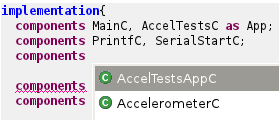
\includegraphics[width=0.5\textwidth]{img/eclipse_compl1.png}
  \caption{Component instantiation completion.}
  \label{fig:first_compl}
\end{figure}

\begin{figure}[h]
  \centering
  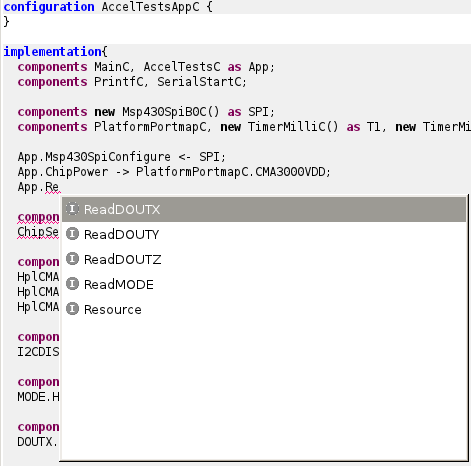
\includegraphics[width=0.55\textwidth]{img/eclipse_compl2.png}
  \caption{User connection completion.}
\end{figure}

Firstly, in the Eclipse editor, the plugin adds {\bf code completion}, which eases writing both module and configuration files. The plugin completes component instantiations and connections. Likewise, it completes interface calls, function calls and variable names, and after adding a \texttt{uses} or \texttt{provides} declaration, it offers to create command and event stubs. These features are best shown in Figures \ref{fig:first_compl} through
\ref{fig:last_compl}.

\begin{figure}[h]
  \centering
  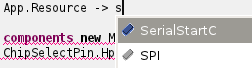
\includegraphics[width=0.45\textwidth]{img/eclipse_compl3.png}
  \caption{Provider connection completion.}
\end{figure}

\begin{figure}[h]
  \centering
  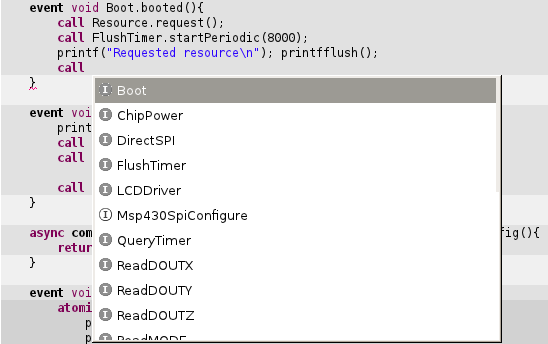
\includegraphics[width=0.6\textwidth]{img/eclipse_compl4.png}
  \caption{Interface completion.}
\end{figure}

\begin{figure}[h]
  \centering
  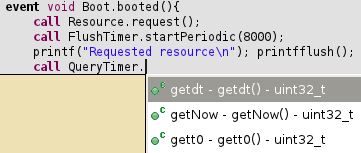
\includegraphics[width=0.64\textwidth]{img/eclipse_compl5.png}
  \caption{Command completion.}
\end{figure}

\begin{figure}[h]
  \centering
  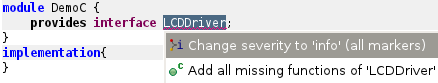
\includegraphics[width=0.72\textwidth]{img/eclipse_compl6.png}
  \caption{Command stubs generation.}
  \label{fig:last_compl}
\end{figure}

Another useful feature, especially for a new developer wishing to familiarize himself with TinyOS, is the {\bf component explorer}. It graphically displays components instantiated and interconnected in configurations. Interfaces can be viewed as well.  Starting at the top-level application configuration, every part of the applications and underlying systems code can be reached. This is by far the most efficient way to explore the call hierarchy and find where particular functions are implemented. The example of the PrintfC configuration, viewed through the component explorer is shown in Figure \ref{fig:eclipse_compexp}.

\begin{figure}[h]
  \centering
  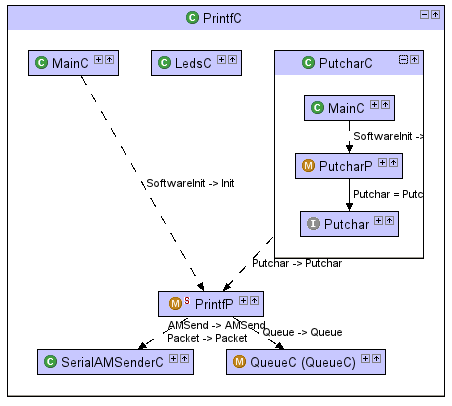
\includegraphics[width=0.7\textwidth]{img/eclipse_compexp.png}
  \caption{Component explorer showing PrintfC configuration.}
  \label{fig:eclipse_compexp}
\end{figure}

The Eclipse editor also gives many warnings about the code without triggering compilation. Moreover, many of these warnings are not raised by the NesC compiler, the \emph{cast to a shorter type} warning.

Finally, one of the most useful parts of Yeti 2 is {\bf the debugger}.  The chain of tool invocations, needed to debug an application on the Chronos watch is long, but running them is as easy as pressing a button in the IDE. At the lowest level, the \emph{mspdebug} communicates with the watch through the USB debugging dongle. It runs a GDB Server to which newer versions of \emph{msp430-gdb} are able to connect. Eclipse runs this last executable and forms practical data views, reading crude data from GDB. The following features seem most useful in practice
\begin{itemize}
  \item Single stepping through code in the NesC editor.
  \item Call stack view.
  \item Breakpoint list (though limited to 3 active at any moment).
  \item Disassembly view.
  \item Raw memory view.
  \item Register view.
  \item Local variable view.
  \item Module variable view.
\end{itemize}

Yeti 2 provides many more functions not mentioned here, most of which are standard for Eclipse IDE and are expected to be available for any supported programming language. A developer can naturally explore them while using the IDE.

A preconfigured setup of the plugin is available in the virtual machine distributed with this work.

\section{Console centric development}

It is also possible to develop TinyOS code without using any IDE.  To support such a style of development, two changes are necessary.  Firstly, the environment variables have to be configured to point to the TinyOS source code locations and Makefile rules. This makes it possible to use the make command to build applications. Secondly, syntax and indentation configurations files for vim can be added to ensure convenient code editing.  Having both, a working make system and a good text editor, allows for almost as efficient a development as with the Eclipse IDE. The only drawback is that, if the developer is not familiar with the TinyOS naming conventions, he won't receive aid from code completion tool.

\section{Development virtual machine}

Setting up the tools needed for the TinyOS Chronos platform, is complicated and takes time. To ease this step for new developers, we have created a dedicated virtual machine image. It contains all the tools, which, in addition are configured to work out-of-the-box. The most recent version of the source code is checked out from the rhoRoute SVN repository and imported into the Eclipse IDE, with a run configuration ready to build and install the sample TinyOS Blink application.  All that is left to the user is connecting the watch through the USB debug interface and pressing the Run button.

% to enable wrapped line navigation:
% map j gj
% map k gk

% vim settings:
% vim: set nonumber:
% vim: set spell:
% vim: set linebreak:
% vim: set wrap:
% vim: set textwidth=0:
% vim: set fo+=t:
